\documentclass{beamer} 
\usetheme[]{Feather} 
\usecolortheme{beaver} 
\usepackage{color} 
\usepackage[T1]{fontenc} 
\usepackage[utf8]{inputenc} 
\let\Tiny=\tiny 
\usepackage{pgfplots}
\pgfplotsset{compat=newest,compat/show suggested version=false} 
\usepackage{pgf-pie}
\usepackage{tikz}
\usepackage{hyperref}
\usepackage{graphicx}
\graphicspath{ {Feathergraphics//} }
\newcommand{\chref}[2]{ \href{#1}{{\usebeamercolor[bg]{Feather}#2}}} 
\title[] {       \textbf{Proyecto 1 - Analizador Léxico}}\subtitle[Analizador Léxico]{\textbf{Compiladores e Intérpretes}}\author[Luis Rojas - Ariel Montero - Bryan Jiménez]{      Luis Rojas - Ariel Montero - Bryan Jiménez \\{\ttfamily IS 2017}}\institute[]{Instituto Tecnológico de Costa Rica\\}\date{\today} 
\begin{document} 
 {\1 \begin{frame}[plain,noframenumbering] \titlepage \end{frame}} \begin{frame}{Contenido}{} \tableofcontents \end{frame} 
\section{Explicación General}\subsection{Datos Generales}\begin{frame}[allowframebreaks] 
\frametitle{Datos Generales} 
 
\begin{block}{\textbf{Definiciones}} 
\textbf{Token}: Familia de lexemas, es una categoría donde se clasifican los lexemas.\newline 
\textbf{Lexema}: Ejemplo particular de la variable.\newline 
\textbf{Hilera}: Cadenas de texto generalmente marcadas entre comillas. \newline 
\textbf{Constante}: Valor que no cambia, ya esta definido. \newline 
\textbf{Identificadores}: Conjunto de caracteres alfanuméricos que sirven para identificar las entidades del programa  \newline 
\end{block}
\begin{block}{\textbf{Definiciones}} 
\textbf{Palabras reservadas}: Palabras que son usadas por el lenguaje y no pueden modificarse ni su función. \newline 
\textbf{Símbolos especiales}: Símbolos con significado especial en el lenguaje por lo que no se pueden usar para  otro proposito.\newline 
\textbf{Operadores}: Símbolos utilizados para realixar operaciones lógicas y matemáticas. \newline 
\end{block}
\end{frame} 
\subsection{Scanning}\begin{frame} 
\frametitle{Scanning} 
 
\includegraphics[width=\textwidth]{scan}\end{frame} 
\begin{frame}[allowframebreaks] 
\frametitle{Scanning} 
 
Un analizador léxico o scanner es la primera fase de un compilador y consistente en un programa que recibe como entrada el código fuente de otro programa (secuencia de caracteres) y produce una salida compuesta de tokens (componentes léxicos) o símbolos. Estos tokens sirven para una posterior etapa del proceso de traducción, siendo la entrada para el analizador sintáctico o parser. La especificación de un lenguaje de programación suele incluir un conjunto de reglas que definen el léxico. Estas reglas consisten comúnmente en expresiones regulares que indican el conjunto de posibles secuencias de caracteres que definen un token o leóxema.\end{frame} 
\subsection{Flex}\begin{frame} 
\frametitle{Flex} 
 
\includegraphics[width=\textwidth]{flex}\end{frame} 
\begin{frame}[allowframebreaks] 
\frametitle{Flex} 
 
Flex es una heramienta para generar scanners, flex lee las entradas para tener una descripción del scanner que debe generar. La descripción se realiza en pares de expresiones regulares y cóodigo en C, que se llaman reglas. Genera una salida en un archivo en C 'lex.yy.c' que define a una rutima 'yylex()'. Este archivo es compilado y unido con la librería '-lfl' para generar el ejecutable. Cuando se llama al ejecutable este analiza la entrada por ocurrencias de las expresiones regulares, cuando encuentra una ejecuta el código correspondiente en C.\end{frame} 
\section{Programa Fuente}\begin{frame}[allowframebreaks] 
\frametitle{Programa Fuente} 
\newline 
\newline 
\newline 
\textcolor{purple}{ int } 
\textcolor{purple}{ main } 
\textcolor{olive}{ ( } 
\textcolor{olive}{ ) } 
\newline 
\textcolor{olive}{ \{ } 
\textcolor{purple}{ int } 
\textcolor{orange}{ cant2 } 
\textcolor{green}{ = } 
\textcolor{blue}{ 0 } 
\textcolor{olive}{ ; } 
\newline 
\textcolor{purple}{ if } 
\textcolor{olive}{ ( } 
\textcolor{orange}{ cant2 } 
\textcolor{green}{ == } 
\textcolor{blue}{ 2 } 
\textcolor{olive}{ ) } 
\textcolor{olive}{ \{ } 
\textcolor{olive}{\} } 
\newline 
\textcolor{purple}{ printf } 
\textcolor{olive}{ ( } 
\textcolor{olive}{ " } 
\textcolor{orange}{ Hola } 
\textcolor{orange}{ mundo } 
\textcolor{olive}{ " } 
\textcolor{olive}{ ) } 
\textcolor{olive}{ ; } 
\newline 
\textcolor{orange}{ x } 
\textcolor{green}{ = } 
\textcolor{blue}{ 2 } 
\textcolor{olive}{ ; } 
\newline 
\textcolor{purple}{ return } 
\textcolor{blue}{ 0 } 
\textcolor{olive}{ ; } 
\newline 
\textcolor{olive}{\} } 
\newline 
\newline 
\textcolor{purple}{ int } 
\textcolor{orange}{ gdc } 
\textcolor{olive}{ ( } 
\textcolor{olive}{ ) } 
\newline 
\textcolor{olive}{ \{ } 
\newline 
\textcolor{purple}{ int } 
\textcolor{orange}{ n1 } 
\textcolor{olive}{ , } 
\textcolor{orange}{ n2 } 
\textcolor{olive}{ , } 
\textcolor{orange}{ i } 
\textcolor{olive}{ , } 
\textcolor{orange}{ gcd } 
\textcolor{olive}{ ; } 
\newline 
\newline 
\textcolor{purple}{ printf } 
\textcolor{olive}{ ( } 
\textcolor{olive}{ " } 
\textcolor{orange}{ Enter } 
\textcolor{orange}{ two } 
\textcolor{orange}{ integers } 
\textcolor{olive}{ : } 
\textcolor{olive}{ " } 
\textcolor{olive}{ ) } 
\textcolor{olive}{ ; } 
\newline 
\textcolor{purple}{ scanf } 
\textcolor{olive}{ ( } 
\textcolor{olive}{ " } 
\textcolor{green}{\%} 
\textcolor{orange}{ d } 
\textcolor{green}{\%} 
\textcolor{orange}{ d } 
\textcolor{olive}{ " } 
\textcolor{olive}{ , } 
\textcolor{green}{\&} 
\textcolor{orange}{ n1 } 
\textcolor{olive}{ , } 
\textcolor{green}{\&} 
\textcolor{orange}{ n2 } 
\textcolor{olive}{ ) } 
\textcolor{olive}{ ; } 
\newline 
\newline 
\textcolor{purple}{ for } 
\textcolor{olive}{ ( } 
\textcolor{orange}{ i } 
\textcolor{green}{ = } 
\textcolor{blue}{ 1 } 
\textcolor{olive}{ ; } 
\textcolor{orange}{ i } 
\textcolor{green}{$<=$} 
\textcolor{orange}{ n1 } 
\textcolor{green}{\&\&} 
\textcolor{orange}{ i } 
\textcolor{green}{$<=$} 
\textcolor{orange}{ n2 } 
\textcolor{olive}{ ; } 
\textcolor{green}{ ++ } 
\textcolor{orange}{ i } 
\textcolor{olive}{ ) } 
\newline 
\textcolor{olive}{ \{ } 
\newline 
\textcolor{purple}{ if } 
\textcolor{olive}{ ( } 
\textcolor{orange}{ n1 } 
\textcolor{green}{\%} 
\textcolor{orange}{ i } 
\textcolor{green}{ == } 
\textcolor{blue}{ 0 } 
\textcolor{green}{\&\&} 
\textcolor{orange}{ n2 } 
\textcolor{green}{\%} 
\textcolor{orange}{ i } 
\textcolor{green}{ == } 
\textcolor{blue}{ 0 } 
\textcolor{olive}{ ) } 
\newline 
\textcolor{orange}{ gcd } 
\textcolor{green}{ = } 
\textcolor{orange}{ i } 
\textcolor{olive}{ ; } 
\newline 
\textcolor{olive}{\} } 
\newline 
\newline 
\textcolor{purple}{ printf } 
\textcolor{olive}{ ( } 
\textcolor{olive}{ " } 
\textcolor{orange}{ G } 
\textcolor{olive}{ . } 
\textcolor{orange}{ C } 
\textcolor{olive}{ . } 
\textcolor{orange}{ D } 
\textcolor{orange}{ of } 
\textcolor{green}{\%} 
\textcolor{orange}{ d } 
\textcolor{orange}{ and } 
\textcolor{green}{\%} 
\textcolor{orange}{ d } 
\textcolor{orange}{ is } 
\textcolor{green}{\%} 
\textcolor{orange}{ d } 
\textcolor{olive}{ " } 
\textcolor{olive}{ , } 
\textcolor{orange}{ n1 } 
\textcolor{olive}{ , } 
\textcolor{orange}{ n2 } 
\textcolor{olive}{ , } 
\textcolor{orange}{ gcd } 
\textcolor{olive}{ ) } 
\textcolor{olive}{ ; } 
\newline 
\newline 
\textcolor{purple}{ return } 
\textcolor{blue}{ 0 } 
\textcolor{olive}{ ; } 
\newline 
\textcolor{olive}{\} } 
\newline 
\newline 
\newline 
\textcolor{purple}{ int } 
\textcolor{orange}{ palindrome } 
\textcolor{olive}{ ( } 
\textcolor{olive}{ ) } 
\newline 
\textcolor{olive}{ \{ } 
\newline 
\textcolor{purple}{ int } 
\textcolor{orange}{ n } 
\textcolor{olive}{ , } 
\textcolor{orange}{ reversedInteger } 
\textcolor{green}{ = } 
\textcolor{blue}{ 0 } 
\textcolor{olive}{ , } 
\textcolor{orange}{ remainder } 
\textcolor{olive}{ , } 
\textcolor{orange}{ originalInteger } 
\textcolor{olive}{ ; } 
\newline 
\newline 
\textcolor{purple}{ printf } 
\textcolor{olive}{ ( } 
\textcolor{olive}{ " } 
\textcolor{orange}{ Enter } 
\textcolor{orange}{ an } 
\textcolor{orange}{ integer } 
\textcolor{olive}{ : } 
\textcolor{olive}{ " } 
\textcolor{olive}{ ) } 
\textcolor{olive}{ ; } 
\newline 
\textcolor{purple}{ scanf } 
\textcolor{olive}{ ( } 
\textcolor{olive}{ " } 
\textcolor{green}{\%} 
\textcolor{orange}{ d } 
\textcolor{olive}{ " } 
\textcolor{olive}{ , } 
\textcolor{green}{\&} 
\textcolor{orange}{ n } 
\textcolor{olive}{ ) } 
\textcolor{olive}{ ; } 
\newline 
\newline 
\textcolor{orange}{ originalInteger } 
\textcolor{green}{ = } 
\textcolor{orange}{ n } 
\textcolor{olive}{ ; } 
\newline 
\newline 
\textcolor{purple}{ while } 
\textcolor{olive}{ ( } 
\textcolor{orange}{ n } 
\textcolor{green}{ != } 
\textcolor{blue}{ 0 } 
\textcolor{olive}{ ) } 
\newline 
\textcolor{olive}{ \{ } 
\newline 
\textcolor{orange}{ remainder } 
\textcolor{green}{ = } 
\textcolor{orange}{ n } 
\textcolor{green}{\%} 
\textcolor{blue}{ 10 } 
\textcolor{olive}{ ; } 
\newline 
\textcolor{orange}{ reversedInteger } 
\textcolor{green}{ = } 
\textcolor{orange}{ reversedInteger } 
\textcolor{green}{ * } 
\textcolor{blue}{ 10 } 
\textcolor{green}{ + } 
\textcolor{orange}{ remainder } 
\textcolor{olive}{ ; } 
\newline 
\textcolor{orange}{ n } 
\textcolor{green}{ / } 
\textcolor{blue}{ 10 } 
\textcolor{olive}{ ; } 
\newline 
\textcolor{olive}{\} } 
\newline 
\newline 
\textcolor{purple}{ if } 
\textcolor{olive}{ ( } 
\textcolor{orange}{ originalInteger } 
\textcolor{green}{ == } 
\textcolor{orange}{ reversedInteger } 
\textcolor{olive}{ ) } 
\newline 
\textcolor{purple}{ printf } 
\textcolor{olive}{ ( } 
\textcolor{olive}{ " } 
\textcolor{green}{\%} 
\textcolor{orange}{ d } 
\textcolor{orange}{ is } 
\textcolor{orange}{ a } 
\textcolor{orange}{ palindrome } 
\textcolor{olive}{ . } 
\textcolor{olive}{ " } 
\textcolor{olive}{ , } 
\textcolor{orange}{ originalInteger } 
\textcolor{olive}{ ) } 
\textcolor{olive}{ ; } 
\newline 
\textcolor{purple}{ else } 
\textcolor{purple}{ printf } 
\textcolor{olive}{ ( } 
\textcolor{olive}{ " } 
\textcolor{green}{\%} 
\textcolor{orange}{ d } 
\textcolor{orange}{ is } 
\textcolor{orange}{ not } 
\textcolor{orange}{ a } 
\textcolor{orange}{ palindrome } 
\textcolor{olive}{ . } 
\textcolor{olive}{ " } 
\textcolor{olive}{ , } 
\textcolor{orange}{ originalInteger } 
\textcolor{olive}{ ) } 
\textcolor{olive}{ ; } 
\newline 
\newline 
\textcolor{purple}{ return } 
\textcolor{blue}{ 0 } 
\textcolor{olive}{ ; } 
\newline 
\textcolor{olive}{\} } 
\newline 
\newline 
\newline 
\textcolor{purple}{ int } 
\textcolor{orange}{ primo } 
\textcolor{olive}{ ( } 
\textcolor{purple}{ int } 
\textcolor{orange}{ n } 
\textcolor{olive}{ ) } 
\textcolor{olive}{ \{ } 
\newline 
\textcolor{purple}{ int } 
\textcolor{orange}{ i } 
\textcolor{olive}{ , } 
\textcolor{orange}{ m } 
\textcolor{olive}{ ; } 
\newline 
\textcolor{purple}{ for } 
\textcolor{olive}{ ( } 
\textcolor{orange}{ i } 
\textcolor{green}{ = } 
\textcolor{blue}{ 2 } 
\textcolor{olive}{ ; } 
\textcolor{orange}{ i } 
\textcolor{green}{\textless} 
\textcolor{orange}{ n } 
\textcolor{olive}{ ; } 
\textcolor{orange}{ i } 
\textcolor{green}{ ++ } 
\textcolor{olive}{ ) } 
\textcolor{olive}{ \{ } 
\newline 
\textcolor{orange}{ m } 
\textcolor{green}{ = } 
\textcolor{orange}{ n } 
\textcolor{green}{\%} 
\textcolor{orange}{ i } 
\textcolor{olive}{ ; } 
\newline 
\textcolor{purple}{ if } 
\textcolor{olive}{ ( } 
\textcolor{orange}{ m } 
\textcolor{green}{ == } 
\textcolor{blue}{ 0 } 
\textcolor{olive}{ ) } 
\textcolor{olive}{ \{ } 
\newline 
\textcolor{purple}{ return } 
\textcolor{blue}{ 1 } 
\textcolor{olive}{ ; } 
\newline 
\textcolor{olive}{\} } 
\textcolor{purple}{ else } 
\textcolor{olive}{ \{ } 
\newline 
\textcolor{purple}{ return } 
\textcolor{blue}{ 0 } 
\textcolor{olive}{ ; } 
\newline 
\textcolor{olive}{\} } 
\newline 
\textcolor{olive}{\} } 
\newline 
\textcolor{olive}{\} } 
\newline 
\newline 
\textcolor{purple}{ int } 
\textcolor{orange}{ armstrong } 
\textcolor{olive}{ ( } 
\textcolor{olive}{ ) } 
\newline 
\textcolor{olive}{ \{ } 
\newline 
\textcolor{purple}{ int } 
\textcolor{orange}{ number } 
\textcolor{olive}{ , } 
\textcolor{orange}{ originalNumber } 
\textcolor{olive}{ , } 
\textcolor{orange}{ remainder } 
\textcolor{olive}{ , } 
\textcolor{orange}{ result } 
\textcolor{green}{ = } 
\textcolor{blue}{ 0 } 
\textcolor{olive}{ , } 
\textcolor{orange}{ n } 
\textcolor{green}{ = } 
\textcolor{blue}{ 0 } 
\textcolor{olive}{ ; } 
\newline 
\newline 
\textcolor{purple}{ printf } 
\textcolor{olive}{ ( } 
\textcolor{olive}{ " } 
\textcolor{orange}{ Enter } 
\textcolor{orange}{ an } 
\textcolor{orange}{ integer } 
\textcolor{olive}{ : } 
\textcolor{olive}{ " } 
\textcolor{olive}{ ) } 
\textcolor{olive}{ ; } 
\newline 
\textcolor{purple}{ scanf } 
\textcolor{olive}{ ( } 
\textcolor{olive}{ " } 
\textcolor{green}{\%} 
\textcolor{orange}{ d } 
\textcolor{olive}{ " } 
\textcolor{olive}{ , } 
\textcolor{green}{\&} 
\textcolor{orange}{ number } 
\textcolor{olive}{ ) } 
\textcolor{olive}{ ; } 
\newline 
\newline 
\textcolor{orange}{ originalNumber } 
\textcolor{green}{ = } 
\textcolor{orange}{ number } 
\textcolor{olive}{ ; } 
\newline 
\newline 
\textcolor{purple}{ while } 
\textcolor{olive}{ ( } 
\textcolor{orange}{ originalNumber } 
\textcolor{green}{ != } 
\textcolor{blue}{ 0 } 
\textcolor{olive}{ ) } 
\newline 
\textcolor{olive}{ \{ } 
\newline 
\textcolor{orange}{ originalNumber } 
\textcolor{green}{ / } 
\textcolor{blue}{ 10 } 
\textcolor{olive}{ ; } 
\newline 
\textcolor{green}{ ++ } 
\textcolor{orange}{ n } 
\textcolor{olive}{ ; } 
\newline 
\textcolor{olive}{\} } 
\newline 
\newline 
\textcolor{orange}{ originalNumber } 
\textcolor{green}{ = } 
\textcolor{orange}{ number } 
\textcolor{olive}{ ; } 
\newline 
\newline 
\textcolor{purple}{ while } 
\textcolor{olive}{ ( } 
\textcolor{orange}{ originalNumber } 
\textcolor{green}{ != } 
\textcolor{blue}{ 0 } 
\textcolor{olive}{ ) } 
\newline 
\textcolor{olive}{ \{ } 
\newline 
\textcolor{orange}{ remainder } 
\textcolor{green}{ = } 
\textcolor{orange}{ originalNumber } 
\textcolor{green}{\%} 
\textcolor{blue}{ 10 } 
\textcolor{olive}{ ; } 
\newline 
\textcolor{orange}{ result } 
\textcolor{green}{ + } 
\textcolor{green}{ = } 
\textcolor{orange}{ pow } 
\textcolor{olive}{ ( } 
\textcolor{orange}{ remainder } 
\textcolor{olive}{ , } 
\textcolor{orange}{ n } 
\textcolor{olive}{ ) } 
\textcolor{olive}{ ; } 
\newline 
\textcolor{orange}{ originalNumber } 
\textcolor{green}{ / } 
\textcolor{blue}{ 10 } 
\textcolor{olive}{ ; } 
\newline 
\textcolor{olive}{\} } 
\newline 
\newline 
\textcolor{purple}{ if } 
\textcolor{olive}{ ( } 
\textcolor{orange}{ result } 
\textcolor{green}{ == } 
\textcolor{orange}{ number } 
\textcolor{olive}{ ) } 
\newline 
\textcolor{purple}{ printf } 
\textcolor{olive}{ ( } 
\textcolor{olive}{ " } 
\textcolor{green}{\%} 
\textcolor{orange}{ d } 
\textcolor{orange}{ is } 
\textcolor{orange}{ an } 
\textcolor{orange}{ Armstrong } 
\textcolor{orange}{ number } 
\textcolor{olive}{ . } 
\textcolor{olive}{ " } 
\textcolor{olive}{ , } 
\textcolor{orange}{ number } 
\textcolor{olive}{ ) } 
\textcolor{olive}{ ; } 
\newline 
\textcolor{purple}{ else } 
\textcolor{purple}{ printf } 
\textcolor{olive}{ ( } 
\textcolor{olive}{ " } 
\textcolor{green}{\%} 
\textcolor{orange}{ d } 
\textcolor{orange}{ is } 
\textcolor{orange}{ not } 
\textcolor{orange}{ an } 
\textcolor{orange}{ Armstrong } 
\textcolor{orange}{ number } 
\textcolor{olive}{ . } 
\textcolor{olive}{ " } 
\textcolor{olive}{ , } 
\textcolor{orange}{ number } 
\textcolor{olive}{ ) } 
\textcolor{olive}{ ; } 
\newline 
\newline 
\textcolor{purple}{ return } 
\textcolor{blue}{ 0 } 
\textcolor{olive}{ ; } 
\newline 
\textcolor{olive}{\} } 
\newline 
\newline 
\newline 
\newline 
\newline 
\newline 
\newline 
\textcolor{purple}{ int } 
\textcolor{purple}{ main } 
\textcolor{olive}{ ( } 
\textcolor{olive}{ ) } 
\textcolor{olive}{ \{ } 
\newline 
\textcolor{purple}{ int } 
\textcolor{orange}{ factorial } 
\textcolor{olive}{ , } 
\textcolor{orange}{ result } 
\textcolor{green}{ = } 
\textcolor{blue}{ 1 } 
\textcolor{olive}{ ; } 
\newline 
\textcolor{orange}{ x } 
\textcolor{green}{ = } 
\textcolor{blue}{ 2 } 
\textcolor{green}{ - } 
\textcolor{blue}{ 3 } 
\textcolor{olive}{ ; } 
\newline 
\textcolor{orange}{ hola } 
\textcolor{green}{ = } 
\textcolor{blue}{ 23 } 
\textcolor{olive}{ ; } 
\newline 
\textcolor{purple}{ if } 
\textcolor{olive}{ ( } 
\textcolor{orange}{ x } 
\textcolor{green}{ == } 
\textcolor{blue}{ 2 } 
\textcolor{olive}{ ) } 
\textcolor{olive}{ \{ } 
\newline 
\textcolor{purple}{ printf } 
\textcolor{olive}{ ( } 
\textcolor{olive}{ " } 
\textcolor{orange}{ Yo } 
\textcolor{orange}{ soy } 
\textcolor{orange}{ Luis } 
\textcolor{olive}{ " } 
\textcolor{olive}{ ) } 
\textcolor{olive}{ ; } 
\newline 
\textcolor{olive}{\} } 
\textcolor{purple}{ else } 
\textcolor{olive}{ \{ } 
\newline 
\textcolor{purple}{ printf } 
\textcolor{olive}{ ( } 
\textcolor{olive}{ " } 
\textcolor{orange}{ No } 
\textcolor{orange}{ soy } 
\textcolor{orange}{ Luis } 
\textcolor{olive}{ " } 
\textcolor{olive}{ ) } 
\textcolor{olive}{ ; } 
\newline 
\textcolor{olive}{\} } 
\newline 
\textcolor{purple}{ int } 
\textcolor{orange}{ ariel } 
\textcolor{green}{ = } 
\textcolor{blue}{ 3 } 
\textcolor{olive}{ ; } 
\newline 
\textcolor{purple}{ int } 
\textcolor{orange}{ bryan } 
\textcolor{green}{ = } 
\textcolor{blue}{ 7 } 
\textcolor{olive}{ ; } 
\newline 
\textcolor{purple}{ while } 
\textcolor{olive}{ ( } 
\textcolor{orange}{ x } 
\textcolor{green}{ != } 
\textcolor{orange}{ bryan } 
\textcolor{olive}{ ) } 
\textcolor{olive}{ \{ } 
\newline 
\textcolor{purple}{ printf } 
\textcolor{olive}{ ( } 
\textcolor{olive}{ " } 
\textcolor{orange}{ NO } 
\textcolor{orange}{ SOY } 
\textcolor{orange}{ BRYAN } 
\textcolor{olive}{ " } 
\textcolor{olive}{ ) } 
\newline 
\textcolor{olive}{\} } 
\newline 
\textcolor{olive}{\} } 
\newline 
\newline 
\section{Diagramas}\subsection{Histograma}\end{frame} 
\begin{frame} 
\frametitle{Histograma} 
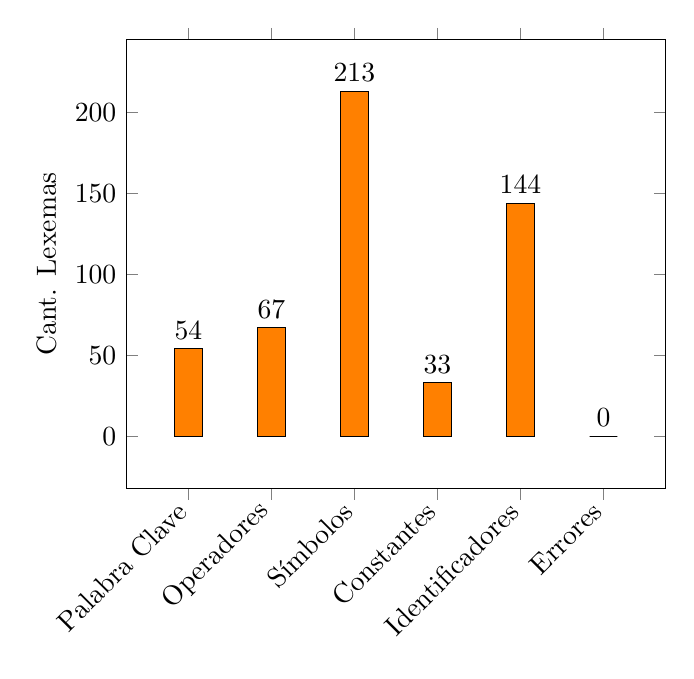
\begin{tikzpicture} 
\begin{axis}[ybar,enlargelimits=0.15,legend style={at={(0.5,-0.2)}, anchor=north,legend columns=-1}, ylabel={Cant. Lexemas},symbolic x coords={Palabra Clave,Operadores,Símbolos,Constantes,Identificadores,Errores},xtick=data,nodes near coords,nodes near coords align={vertical},x tick label style={rotate=45,anchor=east},] 
\addplot[ybar,fill=orange] coordinates {(Palabra Clave,54) (Operadores,67)(Símbolos,213) (Constantes,33) (Identificadores,144) (Errores,0)}; 
\end{axis} 
\end{tikzpicture} 
\end{frame} 
\subsection{Diagrama Pastel}\begin{frame}{Diagrama Pastel} 
\def\angle{0}\def\radius{2}\def\labelradius{3}\def\cyclelist{{"green","purple","red","blue","orange","olive"}}\centering\newcount\cyclecount \cyclecount=-1\newcount\ind \ind=-1\begin{tikzpicture}\foreach \percent/\name in {10/P.Clave.,13/Opera.,41/Símb.,6/Const.,28/Ident.,0/Error} {\ifx\percent\empty\else\global\advance\cyclecount by 1\global\advance\ind by 1\ifnum6<\cyclecount\global\cyclecount=0\global\ind=0\fi\pgfmathparse{\cyclelist[\the\ind]}\edef\color{\pgfmathresult}\draw[fill={\color!50},draw={\color}] (0,0) -- (\angle:\radius) arc (\angle:\angle+\percent*3.7:\radius) -- cycle;\draw[draw=gray, shorten >=2pt] (\angle+0.5*\percent*3.7:\labelradius) node {\name~[\percent\%]} edge (\angle+0.5*\percent*3.7:\radius);\pgfmathparse{\angle+\percent*3.7}\xdef\angle{\pgfmathresult}\fi};\end{tikzpicture}\end{frame} 
{\1\begin{frame}[plain,noframenumbering] \finalpage{\textbf{MUCHAS GRACIAS}}\end{frame}} 
\end{document} 
